%% LyX 1.6.2 created this file.  For more info, see http://www.lyx.org/.
%% Do not edit unless you really know what you are doing.
\documentclass[11pt,letterpaper,twoside,english]{article}
\usepackage[T1]{fontenc}
\usepackage[latin9]{inputenc}
\usepackage{fancyhdr}
\pagestyle{fancy}
\usepackage{babel}

\usepackage{float}
\usepackage{graphicx}
\usepackage[authoryear]{natbib}
\usepackage[unicode=true, pdfusetitle,
 bookmarks=true,bookmarksnumbered=false,bookmarksopen=false,
 breaklinks=false,pdfborder={0 0 0},backref=false,colorlinks=false]
 {hyperref}

%%%%%%%%%%%%%%%%%%%%%%%%%%%%%% User specified LaTeX commands.


\usepackage{fullpage}

\ifx\pdfoutput\undefined
    % we are running LaTeX, not pdflatex
    
\else
    % we are running pdflatex, so convert .eps files to .pdf
    
    \usepackage{epstopdf}
\fi

\author{Yizhi Cai \& Chris Lasher}
\title{GBCB 5874 Final Paper: Jelesko Pathway Evolution Database}
\date{May 6, 2009}

\usepackage{fancyhdr}
\setlength{\headheight}{15pt}

\lhead{GBCB 5874 Final Paper}
\rhead{Cai \& Lasher}

\begin{document}

\title{GBCB 5874 Final Paper: Jelesko Pathway Evolution Database}


\author{Yizhi Cai, Chris Larsher\\
Supervised by Dr. John Jelesko}


\date{2009-05-09}

\maketitle

\section{Introduction}

%
\begin{figure}[h]
\begin{centering}
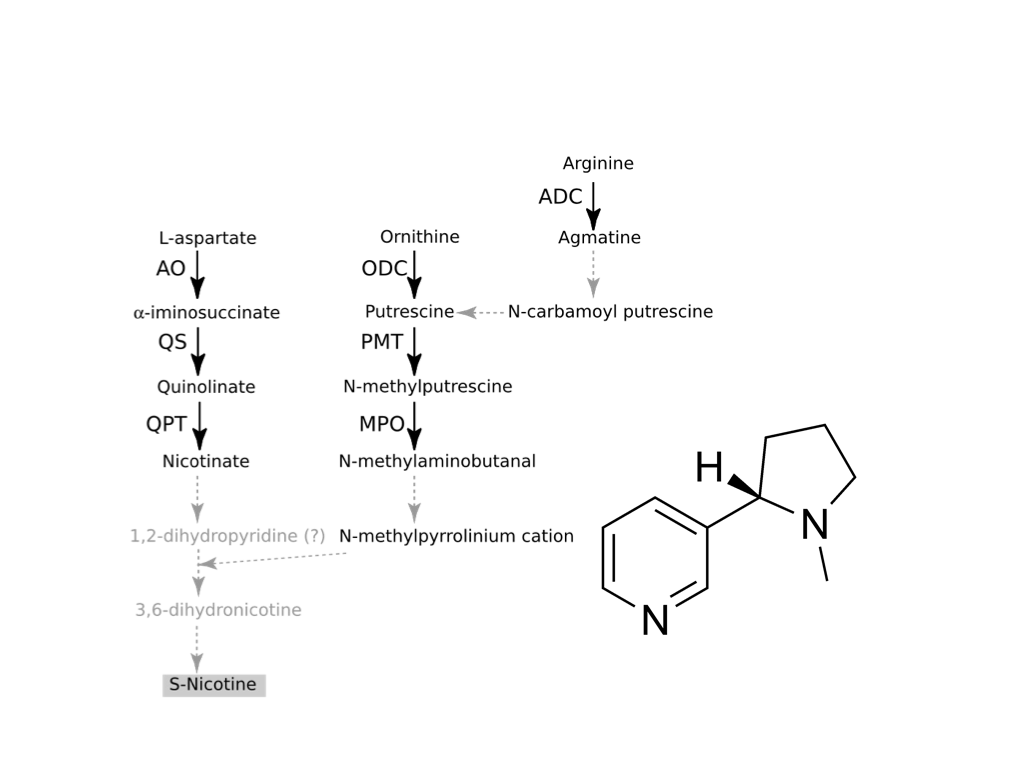
\includegraphics[width=1\linewidth]{figures/Nicotine_pathway}
\par\end{centering}

\caption{Nicotine pathway}

\end{figure}


%
\begin{figure}[h]
\begin{centering}
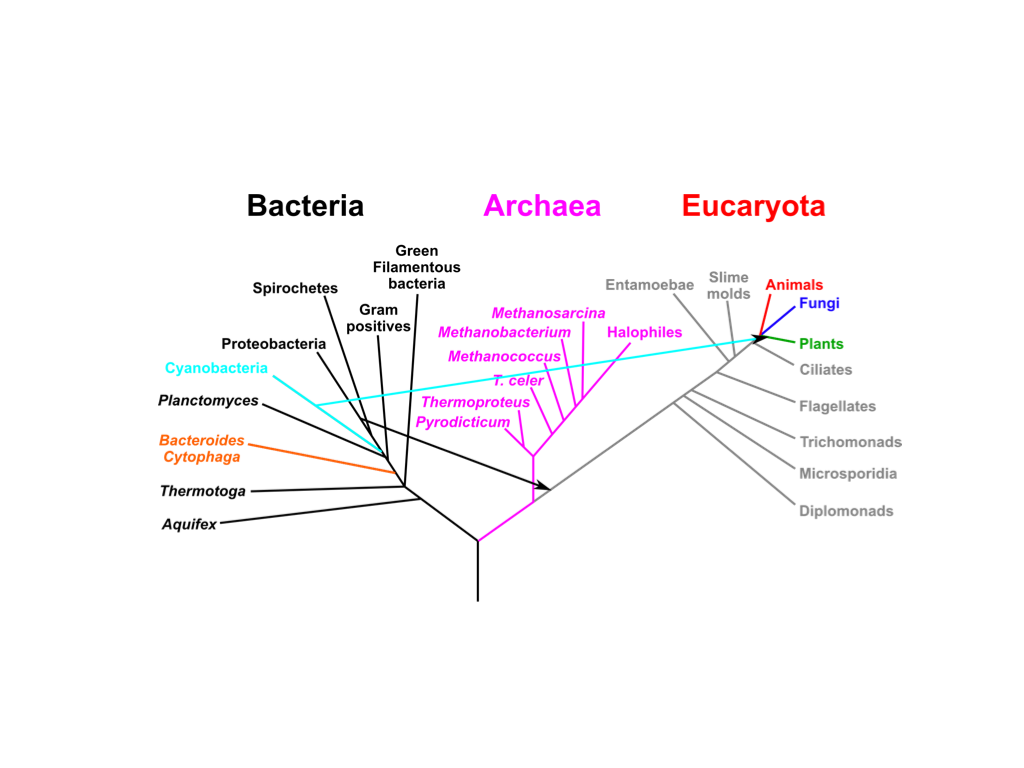
\includegraphics[width=1\linewidth]{figures/Tree_of_life}
\par\end{centering}

\caption{Tree of life}

\end{figure}



\section{Methods}

Figure \ref{fig:The-workflow-of} shows the overall workflow of this
project. The whole project is database driven and composed of three
major components. The first component is Data acquisition, which needs
to fetch sequence data from NCBI and JGI using python scripts, and
integrate those data into a local MySQL database. The second major
component is user interfaces developed using Django framework, which
takes a protein sequence in FASTA format and user-specified parameters
to run homology search. Users can select hits of interests to download,
and this will link to the third major component of this project: the
user-specified output functionality. This component takes user-selected
gi numbers to query taxonomic information from the MySQL database
and provides users with output files in different formats. 

% overall pipeline figure goes here


%
\begin{figure}[h]
\begin{centering}
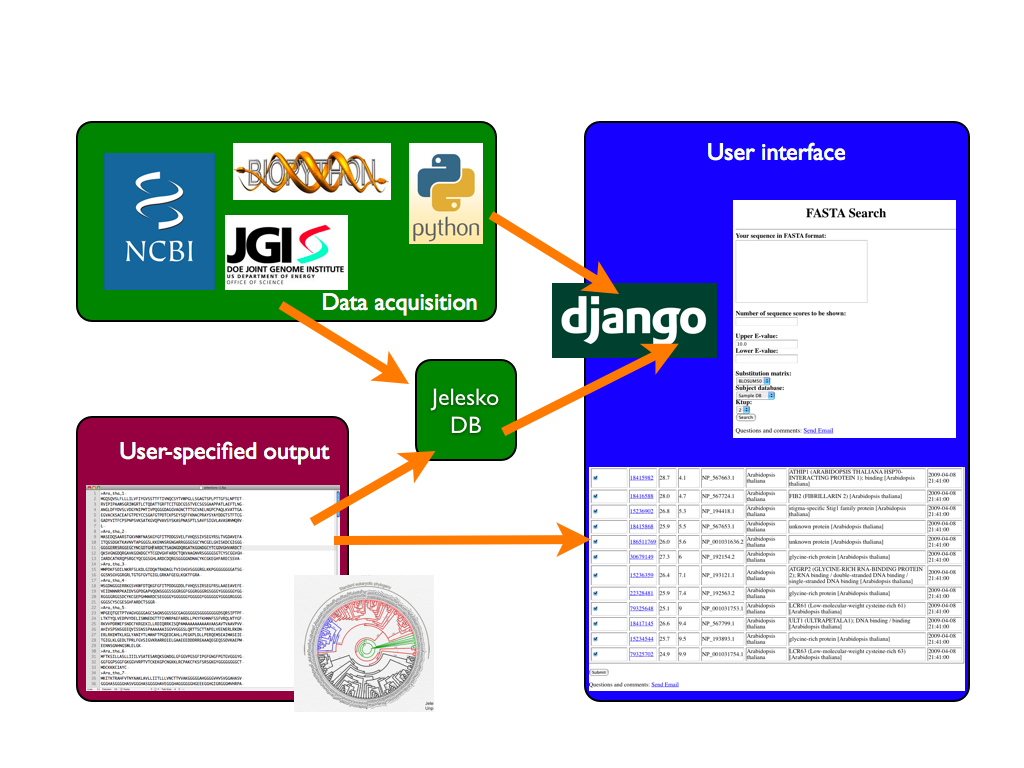
\includegraphics[width=1\linewidth]{figures/work_flow}
\par\end{centering}

\caption{\label{fig:The-workflow-of}The workflow of this project}

\end{figure}



\subsection{\label{sub:Data-Retrieval}Data Retrieval}

% Chris



\subsection{Data Integration}

% Chris



\subsection{Web Interface}

% Patrick   
<<<<<<< HEAD:paper/final_paper.tex

% Describe the design rationable

% Describe data models
=======
>>>>>>> master:paper/final_paper.tex


<<<<<<< HEAD:paper/final_paper.tex
% Patrick 

% Compare BLAST and FASTA/Ssearch algorthms  

% Describe the Biopython module for BLAST

% Describe the customized parser for FASTA and SSearch
=======
% Describe the design rationable


% Describe data models


Figure \ref{fig:Web-interface} outlines the web interface for running
FASTA search. There are three sections of this page. On the top of
the page, there is a sequence input diagram, which takes input sequence
in FASTA format. In the middle of the page, parameters can be specified
as necessary for running homology searches. These parameters include
the number of hits to return, the lower and upper e-value cutoffs,
substitution matrix, and the subject database to search against. Before
sending the input sequence and parameters to run search, it is important
to check the validity of those inputs. The validation includes non-empty
input of sequence, non-negative value of number of hits, and so on.
The validation increases the robustness of the entire web application. 

Once input sequence and user-specified parameters have been validated,
homology searches will be run in the backend. Outputs of the searches
will be interpreted using customized parser and Biopython modules
(see section \ref{sub:Integration-with-FASTA} for implementation
detail). The parsing result include the gi\_number, bit score and
e-value of each hit. And then we use the gi\_number to query the MySQL
database to pull out additional information, which includes accession,
geneus species, annotation and download date of each hit. Finally,
all the information is integrated and render in a nice representation
(see Figure \ref{fig:Homology-search-result}). Users can check certain
hits they are interested in to take a closer look. We also provide
checkall/uncheck all functionality by intergrating a java script. 

Once a user specifies the hits to download, he/she will be redirected
to a download Page (see Figure \ref{fig:Users-selected-files}). The
implementation of the output functionality will be discussed in depth
in section \ref{sub:Output-Generation}. In the download page, there
are three files to be downloaded. The first file is the output file
generated by the homology search, which includes detail alignment
information of the search. The second file is a file containing all
selected sequences in FASTA format. And finally, the last file is
a file that maps internal-used Jelesko-ids to gi numbers.

%
\begin{figure}[h]
\begin{centering}
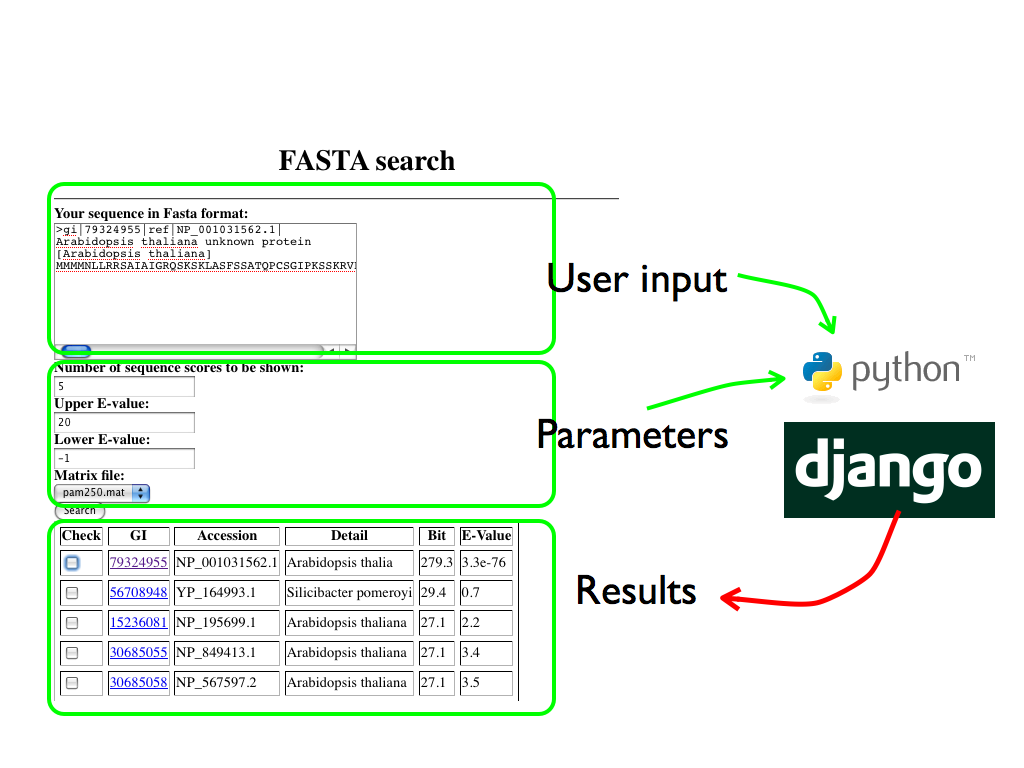
\includegraphics[width=1\linewidth]{figures/web_interface}
\par\end{centering}

\caption{\label{fig:Web-interface}Web interface}

\end{figure}

>>>>>>> master:paper/final_paper.tex

%
\begin{figure}[h]
\begin{centering}
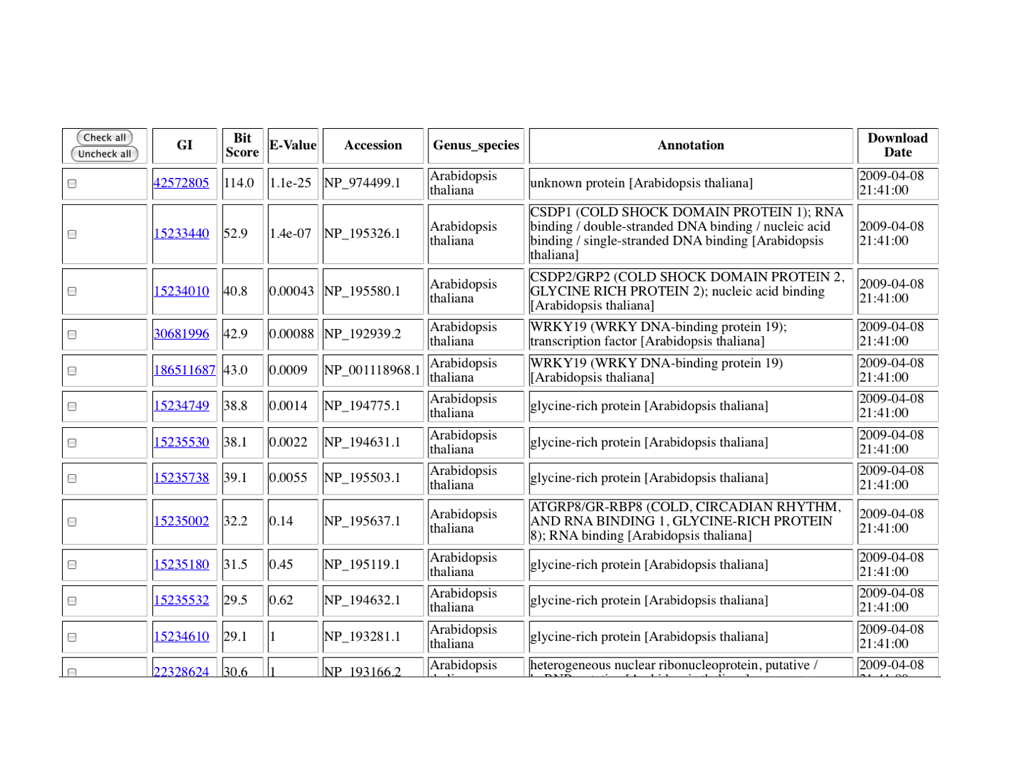
\includegraphics[width=1\linewidth]{figures/Result_selection}
\par\end{centering}

\caption{\label{fig:Homology-search-result}Homology search result}

\end{figure}


%
\begin{figure}[h]
\begin{centering}
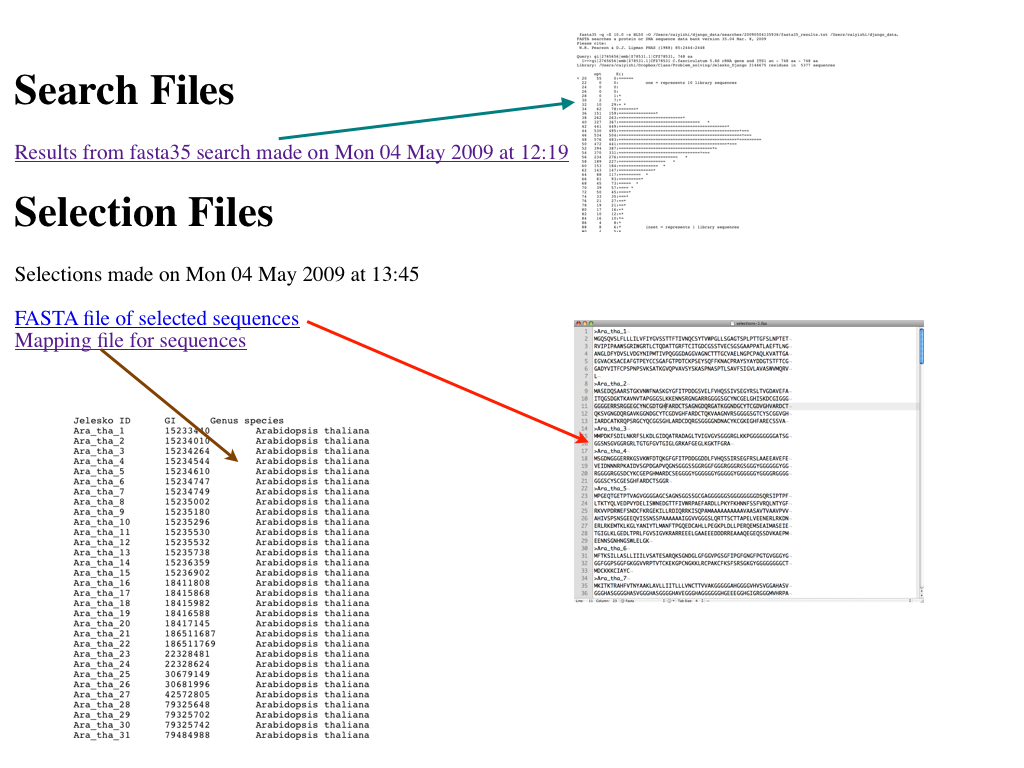
\includegraphics[width=0.8\linewidth]{figures/User_selection}
\par\end{centering}

\caption{\label{fig:Users-selected-files}Users selected files download}

\end{figure}


The web site is built using Django, which is a Python driven framework
for rapid web development. Figure \ref{fig:Django-framework} shows
how Django works. The module of data model is used to interact with
various of databases, in our case, MySQL. Django provides a nice administrator
interface to add/delete entries in the database. The URL configuration
module is used to interpret input URL requests and map them to specific
functions in the view module. The view module is the core component
of the whole framework: it contains a list of functions to process
data from the data model according to the request from the URL module.
After the data has been processed, it will be render with HTML templates. 

%
\begin{figure}[h]
\begin{centering}
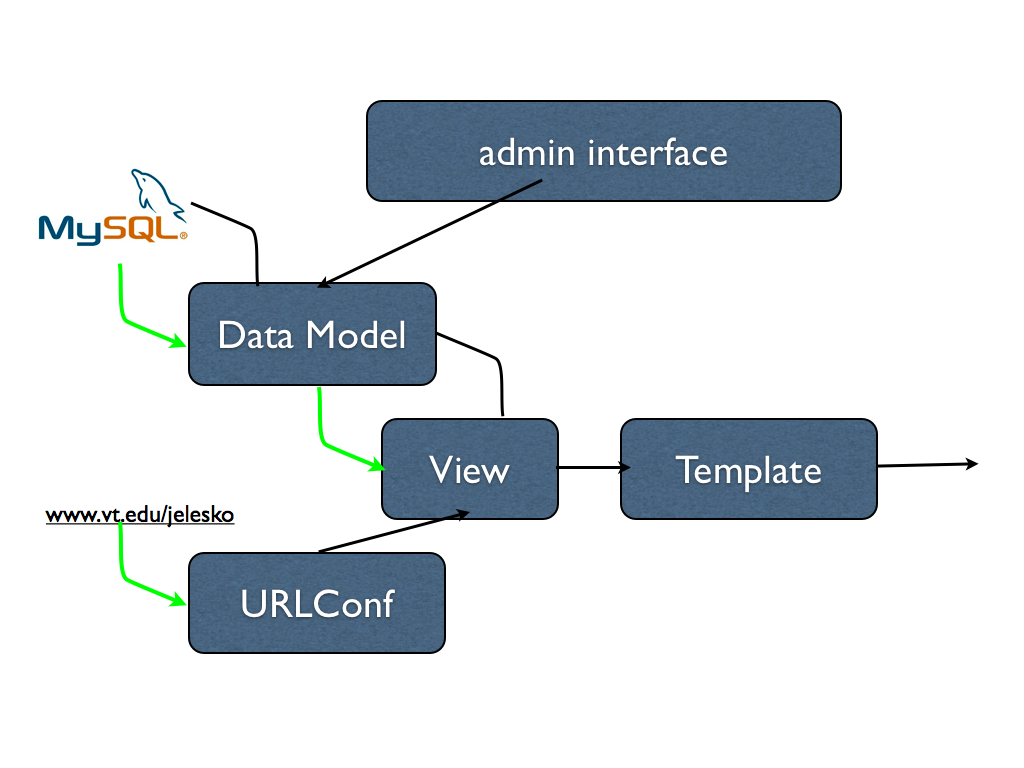
\includegraphics[width=0.6\linewidth]{figures/Django}
\par\end{centering}

\caption{\label{fig:Django-framework}Django framework}

\end{figure}



\subsubsection{\label{sub:Integration-with-FASTA}Integration with FASTA and BLAST}

%
\begin{figure}[H]
\begin{centering}
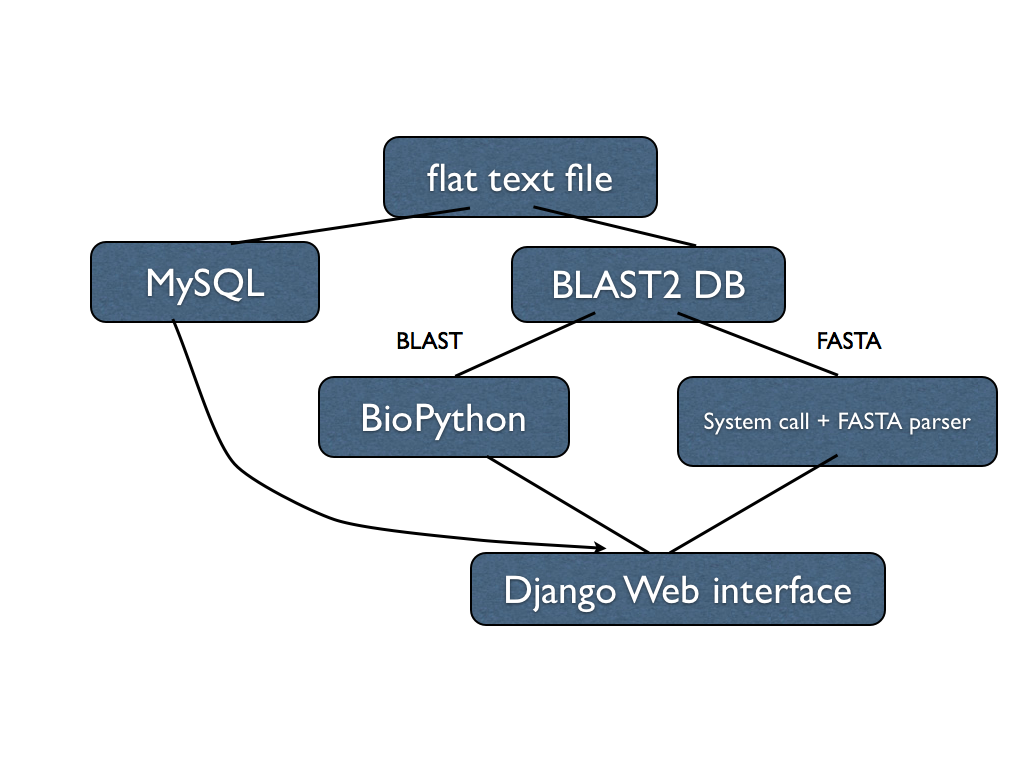
\includegraphics[width=0.7\linewidth]{figures/Data_flow}
\par\end{centering}

\caption{\label{fig:Integration-with-FASTA}Integration with FASTA and BLAST}

\end{figure}


Sequences database similarity search algorithms include two major
categories: algorithms based on dynamic programming and algorithms
based on heuristic algorithms. Widely used dynamic programming based
algorithms include Needleman-Wunsch algorithm and Smith-Waterman algorithm.
BLAST and FASTA are both based on heuristic algorithm. Generally speaking,
BLAST is faster than FASTA while FASTA outperforms BLAST in terms
of sensitivity. A benchmark comparison of BLAST and FASTA is described
in section \ref{fig:Benchmark-result}.

To enjoy the advantages of both, we need to integrate BLAST and FASTA.
After the data retrieve and integration steps, we got a giant flat
text file containing 4 million sequence data. This text file has been
imported as a table in MySQL database, and also been converted into
BLAST2 database format using formatdb command. Both BLAST and FASTA
search programs recognize the BLAST2 format. For running BLAST search,
we leveraged to use the BLAST module of Biopython \citet{Cock:2009p22197},
and also used the built-in parse to process the output XML files.
Since there is no available modules for running FASTA and parsing
its output, we decided to use system call to run FASTA program and
save its output in the format of text file. Then a custom parser has
been implemented to process the output text file. The parsed output
of BLAST and FASTA includes a gi number, e-value and bit scores of
each hit. Then we developed scripts to query the MySQL database using
the gi numbers. The intergrated information finally is sent to the
Django web interface. 

% Patrick 


% Compare BLAST and FASTA/Ssearch algorthms  


% Describe the Biopython module for BLAST


% Describe the customized parser for FASTA and SSearch



\subsubsection{\label{sub:Output-Generation}Output Generation}

% Patrick



\section{Results}

% ? Not sure about this yet. Would be nice if we could prove a use case.

<<<<<<< HEAD:paper/final_paper.tex
% Compare the number of hits in these regions: 0 ~ 10^-20, 10^-20 ~ 10^-2

\section{Conclusions}
=======

% Compare the number of hits in these regions: 0 ~ 10^-20, 10^-20 ~ 10^-2


In order to illustrate the application of this project, we used three
protein sequences (namely A622, NtNUP1 and NtMPO1) to benchmark three
homologous searches. Figure \ref{fig:Benchmark-result} presents the
benchmark result in terms of computation time and search sensitivity.
Searches are performed against the complete database, which contains
4 million sequences. The result suggests that both FASTA and Ssearch
are more computationally expensive than BLAST, but both obtain more
hits than BLAST. Also, we observe that with the close computational
time, Ssearch outperforms FASTA, especially in the case of A622. 

%
\begin{figure}[H]
\begin{centering}
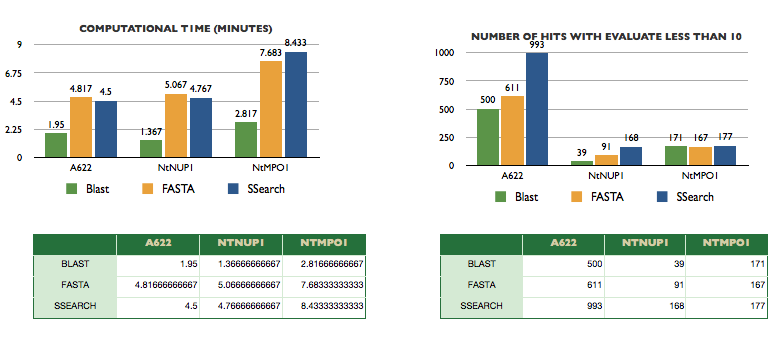
\includegraphics[width=0.8\linewidth]{figures/Bench_mark_result}
\par\end{centering}

\caption{\label{fig:Benchmark-result}Benchmark result}

\end{figure}



\section{Summaries and future workflow}

We began this project from scratch, and by the end of the semester
we have completed the project by accomplishing these tasks:
\begin{enumerate}
\item We have fetched more than 4 million sequences from NCBI, JGI and other
sources.
\item We have developed custom parser for interpreting FASTA outputs, and
leveraged BioPython for data integration. 
\item We have created MySQL, BLAST and FASTA databases for data storage. 
\item We have built web interface for running BLAST, FASTA and Ssearch homology
searches. 
\item We also have implemented user-specified output functionality. 
\end{enumerate}
We envisage and would like to suggest a few future work for the continuation
of the project. First, additional sequence data should be retrieved
from NCBI. Second, we need to incorporate sequences from JGI and other
sources. Last, it will be helpful to save web searches for later reviewing. 


\section{Acknowledgements}

YC and CL would like to thank Dr.John Jelesko for overseeing the project
and giving valuable supervision, Dr's David Bevan and Alexey Onufriev
for teaching this class, and Alexander James Weisberg for assistance
on Linux administration. 

\bibliographystyle{IEEEtran}
\bibliography{Bio}
>>>>>>> master:paper/final_paper.tex

\end{document}
